\documentclass{article}

\usepackage{graphicx}
\usepackage{verbatim}
\usepackage{amssymb}
\usepackage{amsmath}
\usepackage{hyperref}
\usepackage{authblk}

\setlength\itemsep{1em}
\hyphenation{E-the-re-um at-tes-ta-tion}

\title{The Attestation Aggregation\\and Packing Problem}
\author{Satalia \& Sigma Prime}

\begin{document}

\maketitle{}

\begin{abstract}
The Attestation Aggregation and Packing Problem (AAPP) arises in the context of
Ethereum's Proof of Stake (PoS) consensus protocol. This document aims at
formally defining the problem. This will provide the necessary level of detail
needed to develop optimisation algorithms and state properties of them, if
necessary.

Lighthouse, Sigma Prime's Ethereum consensus client, uses a greedy heuristic to
generate solutions to the AAPP. The goal of the present investigation is to
assess how far the solutions generated by Lighthouse's greedy heuristic are
from the real optimum. Ultimately, the goal is to confirm that the current
algorithm is sufficiently good, or to develop an algorithm that produces more
profitable solutions.
\end{abstract}

\tableofcontents

\section{Background}

This section aims to provide a high-level discussion of some concepts behind
blockchain technology those relevant to understand the AAPP.

\subsection{Decentralised trustless architecture}

At its core, a blockchain is a database designed to be tamper-proof. Unlike
other technologies which rely on \emph{trusted central authorities} to
guarantee the integrity of the stored data, a blockchain achieves the same goal
using a \emph{decentralised trustless architecture}. 

This decentralised trustless architecture is based on a combination of
\emph{cryptography}, which allows every participant in a blockchain to
independently verify the integrity of the stored data, and \emph{consensus
protocols}, which allow participants to reliably agree on what ``history'' of
the blockchain is the correct one. This necessity to agree on the history of
the blockchain is a side effect of the distributed nature of the blockchain,
which means that the participants' view of the blockchain can become out of
sync.

\subsection{Blocks and chains}

The blockchain is the historical record of the transactions happened so far.
Transactions are grouped into blocks, and valid blocks become part of the
history when they are appended. Because of the lack of a centralised authority,
any participant can virtually produce a block and broadcast it to the rest of
the participants. 

\subsection{Consensus protocols}

Consensus protocols are rules that all participants in a blockchain must
respect. Such protocols are designed to provide incentives for participants to
do useful work for the blockchain (e.g., producing new blocks, recording new
transactions), and to protect the blockchain from attacks that aim at rewriting
the blockchain's history.  Participants who play by the rules are rewarded by
the protocol, and participants who don't are penalised. In this section we give
an overview of the two main types of consensus protocols: Proof-of-Work and
Proof-of-Stake.  We cover the former for historical reasons, and the latter
because it's the context for the AAPP.

\subsubsection{Proof-of-Work}

A Proof-of-Work (PoW) consensus protocol discourages tampering by making it
unreasonably hard to modify the history of the blockchain. In order to produce
a state change, a participant needs to demonstrate that they have carried out
some \emph{work} that is expensive and cannot be avoided. While doing the work
is hard, verifying that that work has been done is trivial.

Many blockchains, including Bitcoin and Ethereum, are based on PoW consensus
protocols.

\subsubsection{Proof-of-Stake}

In a Proof-of-Stake (PoS) consensus protocol discourages bad behaviors by
requiring that participants put forward, or \emph{stake}, a large (fixed) sum
of native cryptocurrency in order to earn the right to produce a block. If a
participant performs legitimate work, they get rewarded with some of the native
currency, but if they fail to do so, they lose the resources that they have
staked. The upcoming new version of Ethereum's consensus protocol is of this
kind.

\subsubsection{Incentives}

Due to the fact that it relies on a distributed trustless architecture, a
blockchain requires participants to carry out useful work, e.g., producing new
valid blocks, and to avoid disruptive behavior, e.g., tampering with the
blockchain history.  To this end, consensus protocols make extensive use of
(positive or negative) reward mechanisms to incentivise participants to align
with the interests of the chain. Rewards are quantified in a native
cryptocurrency, e.g., Bitcoin, Ether, etc.

\subsection{Agreeing on one history}

The distributed nature of the blockchain leads to some more complications.
Because participants can produce and share new blocks all the time, the chain
doesn't always look like a linear \emph{sequence of blocks}. For instance, two
participants may produce two ``competing'' blocks with the same predecessor,
resulting in a \emph{tree of blocks}.  

The trouble with trees of blocks is that each branch of the three corresponds
to a different ``truth'' about the state of the blockchain, which needs to be
reconciliated in order for the chain to operate correctly and efficiently.
From the perspective of the participants, this means agreeing on which branch
of the tree represents the real truth. Blocks that are not part of such branch
are called \emph{uncle blocks}. 

\subsubsection{Longest chain}

In some blockchains, a convention among the participants is that, in presence
of a tree of blocks, the \emph{longest branch} of the tree represents the one
true history. In order to incentivise participants to commit to the longest
branch, consensus protocols reward block producers asymmetrically, i.e.,
non-uncle blocks are rewarded significantly more than uncle blocks.

\subsubsection{Voting on one history}

Aside from the introduction of Proof-of-Stake, Ethereum's new consensus
protocols introduces some novelties also around the mechanism to agree on the
true history of the blockchain. Instead of adopting the longest branch as the
one true blockchain, \emph{validators}, i.e., participants who agreed to stake
their currency and provide services to the blockchain, cast a vote to elect
(among other things) what they believe is the \emph{head}, i.e., the latest
block of the correct branch, of the blockchain.

Such ``votes'' are called \emph{attestations}, and are the subject of the AAPP
defined in this document.

\section{Attestations in Ethereum}

As discussed in the previous section, a validator vote for the head of the 
chain by producing an attestation. A fundamental property of attestations is
that, under certain conditions they can be aggregated.

An attestation is defined by the following data
%
\begin{itemize}
  \item a set of \textbf{attesters} (possibly 1) that ``back'' it, 
  \item some \textbf{attestation data} (among other things, the slot in which
  the attestation was produced, the hash of the block believed to be the head
  of the chain, and the hashes of two - source and destination - blocks, which
  are related to the mechanism by which older parts of the blockchain are
  finalised), 
  \item a Boneh–Lynn–Shacham (BLS) \textbf{signature} produced using the
  private keys of the attesters.  
\end{itemize}
%
The signature allows to verify the integrity of an attestation. Moreover, a
crucial property of the BLS signature scheme is that it allows to
\emph{aggregate} multiple signatures into a single signature. This allows one
to aggregate multiple attestations into a single one. In order for two
attestations to be aggregated, the following conditions must hold
%
\begin{enumerate} 
  \item their attestation data must be identical, 
  \item their sets of attesters must be disjoint.
\end{enumerate}
%
An aggregated attestation can contain a \textbf{maximum of 2048} attesters.

\subsection{Epochs, slots, committees}

Time in Ethereum is split in successive \emph{epochs} of 6.4 minutes.  Each
epoch is further split into 32 \emph{slots} of 12 seconds. Each block has a
corresponding slot, however not all slots necessarily have a corresponding
block. In fact, there should be only one block per slot, and validators are
penalised for proposing more than one.

At each epoch one validator (the \emph{proposer}) is selected\footnote{Since
we're operating in a decentralised and trustless context, nobody is actually
``selecting'' a validator to propose a block. Instead, the validators will
independently and deterministically derive their role based on the agreed state
of the blockchain.} to propose a new block at a given slot. When its assigned
slot starts, the proposer has a chance to produce a block.

At each epoch, the validators are shuffled and grouped into \emph{committees}.
Each committee has $n \in \left[128, 2048\right]$ validators. A slot has $m \in
\left[1, 64\right]$ committees. The majority of the validators in a committee
become \emph{attesters} and will have to produce an attestation. Among these a
small amount, on expectation 16, will become \emph{aggregators} and will have
to aggregate attestations. 

\subsection{Timeline}

This section gives a brief overview of the timelines involved. These are not
crucial to the problem formulation, but help understanding where the problem
comes from, and why there is only a very limited amount of time available to
solve it.

At each epoch, the work of each validator (be it a proposer, an attester, or an
aggregator) needs to be carried out in the time of the slot assigned to them.
The time before and after the assigned slot is still used to do useful work,
mostly around gathering information, or finishing work that wasn't completed on
time.

Before the start of their assigned slot, a \textbf{proposer} will start
gathering attestations produced up to 32 slots earlier, as well as
transactions, to include in the block. When the slot starts, the proposer will
produce and share the block as quickly as possible, to maximise the likelihood
that it will be considered by the attesters.

The \textbf{attesters} will wait for the block to be received, or up to 4
seconds from the start of the slot, and then make a decision on the head of the
block. Depending on their \emph{fork choice rule}, they may choose the newly
created block, the block produced at the previous slot, or some other block.  
Within 8 seconds from the start of the slot, they will send their attestation
to a sub-network where aggregators are listening for attestations.

\textbf{Aggregators} will gather all the attestations, and try to aggregate as
many as possible into one. Before the end of the slot,
the aggregators will broadcast the aggregated attestations with the network.  
These aggregated attestations (and possibly some unaggregated ones) will be
then gathered by the proposer of the next slot, in a continuous loop.

The diagram in Figure \ref{fig:timeline} summarises the above timeline.
%
\begin{figure}[!ht]
  \hspace*{-0.1\textwidth}
  \centering
  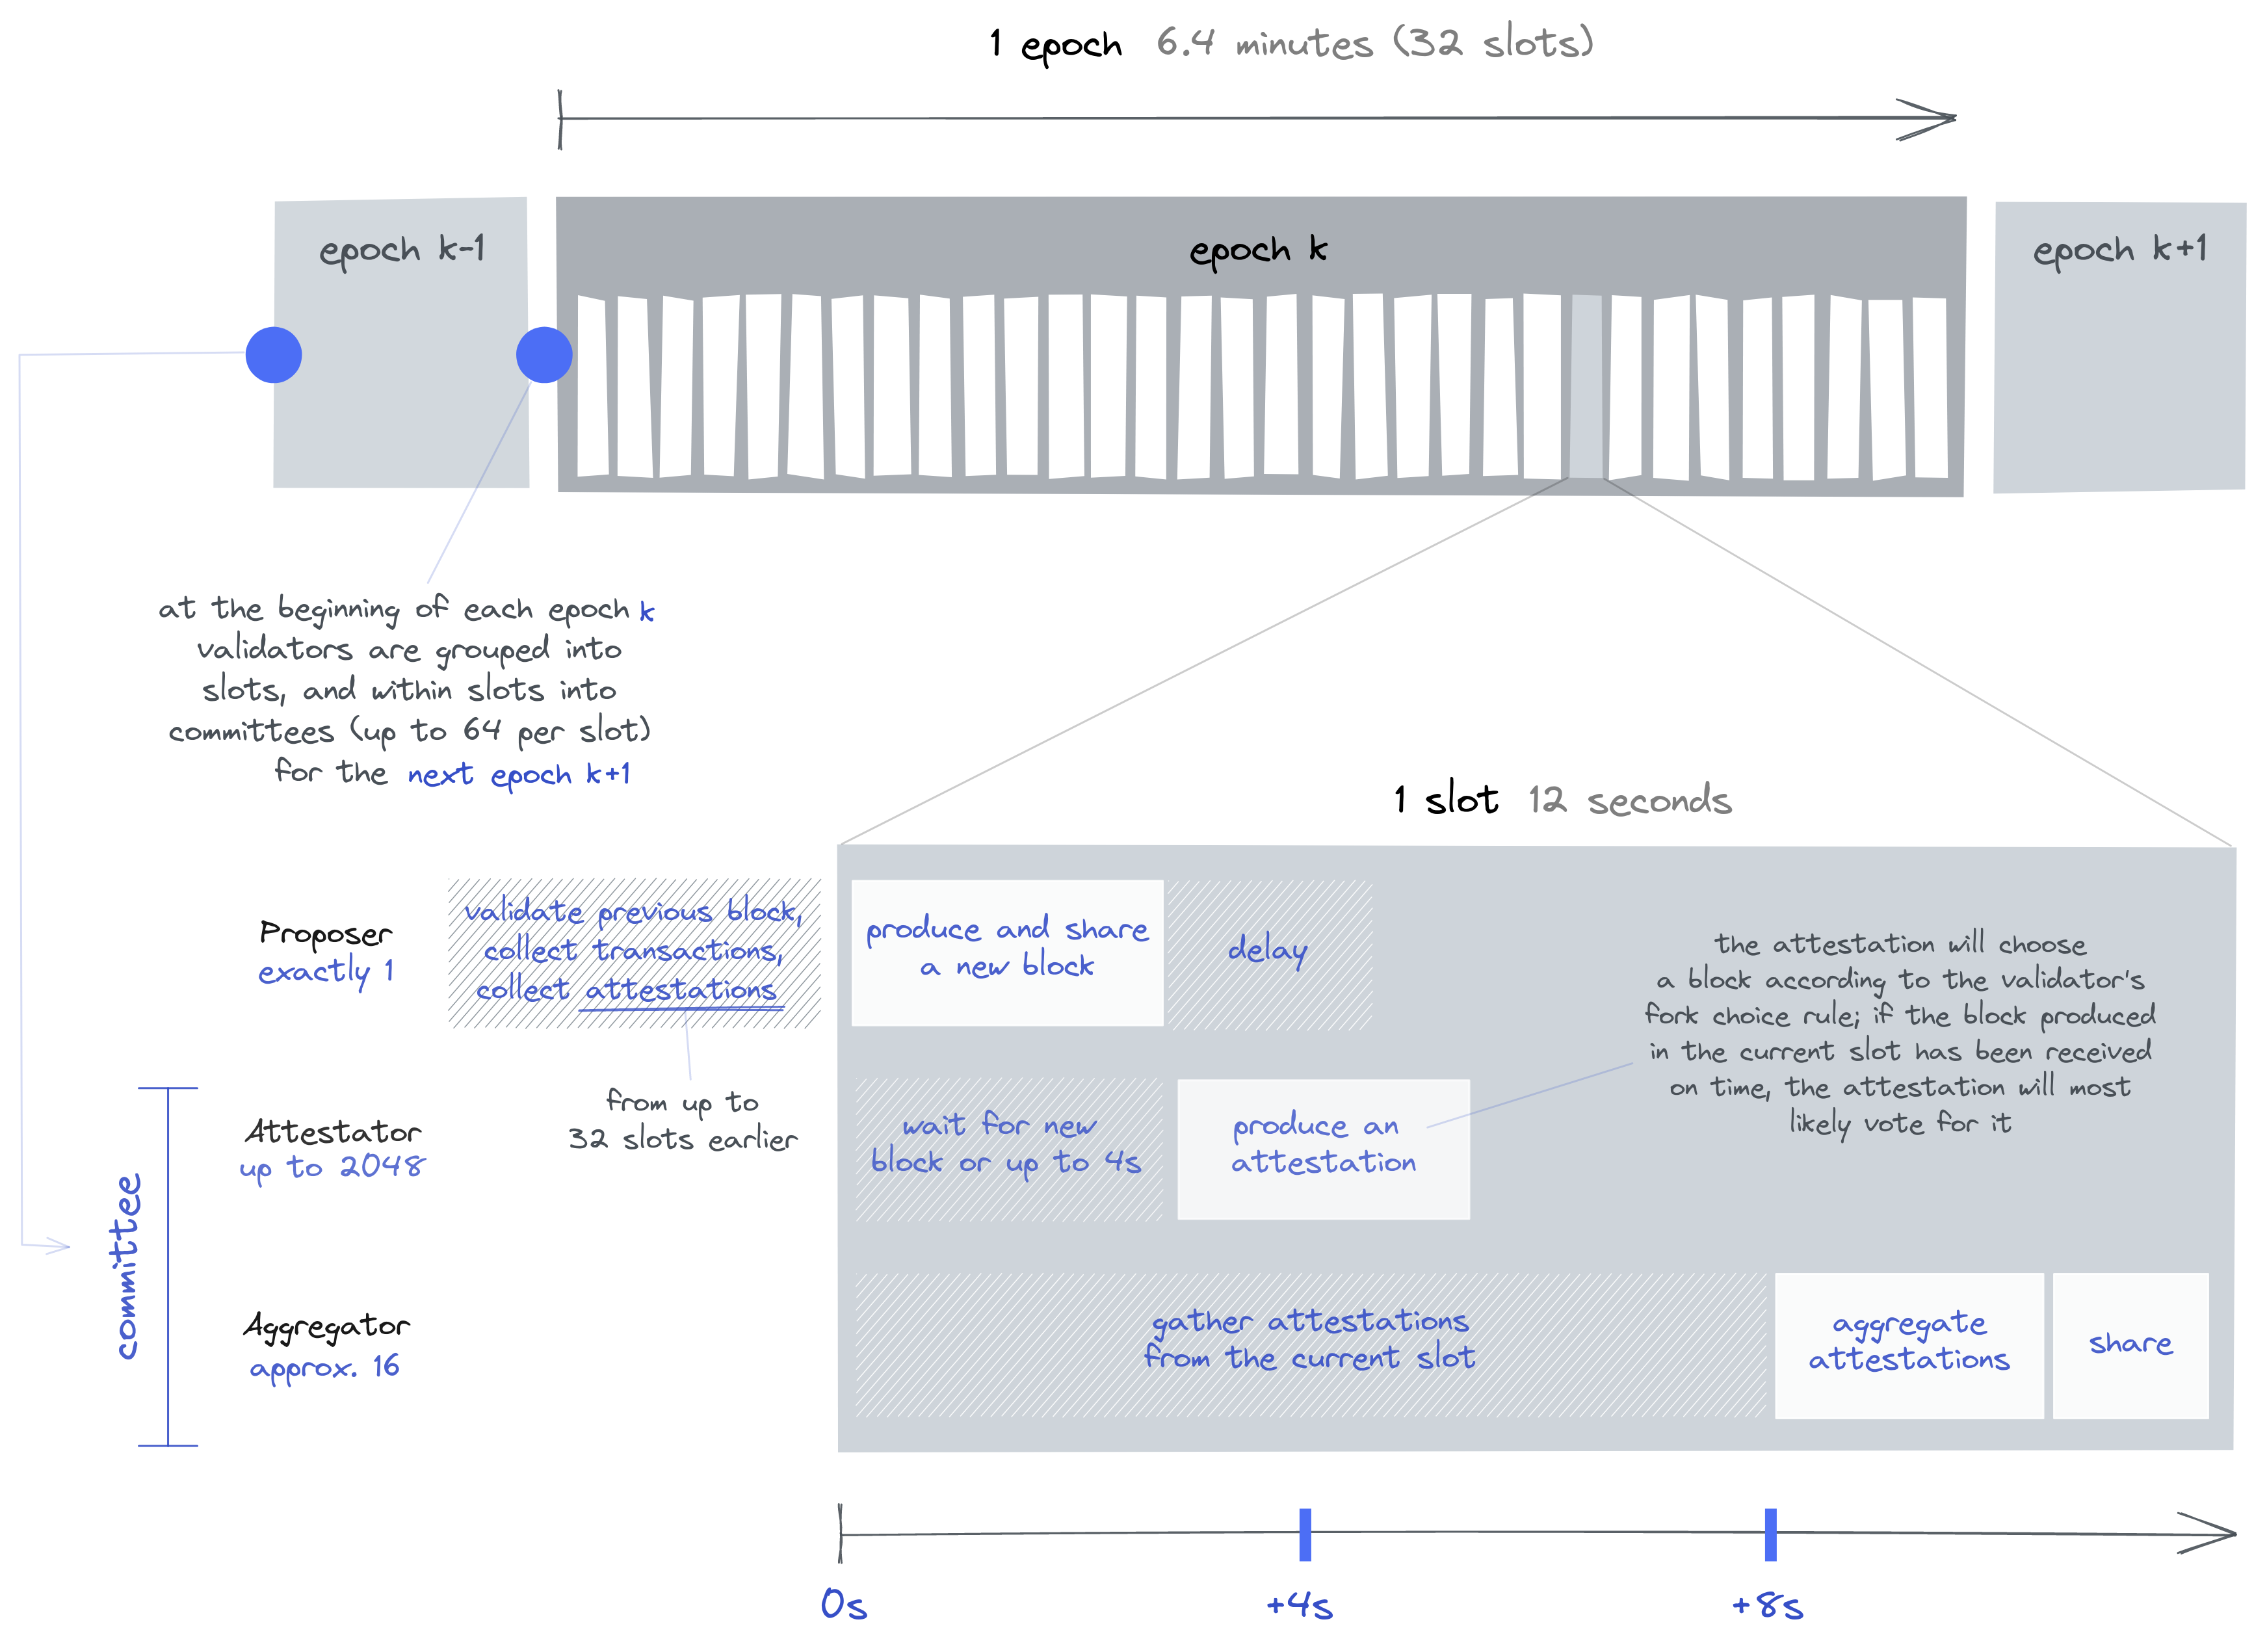
\includegraphics[width=1.2\textwidth]{timeline.png}
  \caption{Timeline for the work of proposers, attesters, and 
  aggregators.\label{fig:timeline}}
\end{figure}

\section{The Attestation Aggregation and Packing Problem}

As covered in the previous section, one key responsibility of the proposer is
to collect attestations from the network, bundle them into a block (along with
transactions), and then share the newly minted block with the network.  Because
the space in a block is limited, the proposer faces the problem of deciding
\emph{which} attestations to include in their block. Moreover, because
different attestations contribute differently to the efficient operation of the
blockchain, and because some attestations have overlaps, the problem of
choosing a set of attestations to include is an \emph{optimisation} problem.
The problem is known as the Attestation Aggregation and Packing Problem (AAPP),
and this section provides a more formal definition for it in terms of entities,
constraints, and objectives.

\newcommand{\attestations}{\ensuremath{A}}
\newcommand{\solution}{\ensuremath{S}}
\newcommand{\attester}{\ensuremath{v}}
\newcommand{\attesters}[1]{\ensuremath{V_{#1}}}
\newcommand{\allattesters}{\ensuremath{V}}
\newcommand{\epoch}[1]{\ensuremath{e(#1)}}
\newcommand{\positives}{\ensuremath{\mathbb{N}^{>0}}}
\newcommand{\block}{\ensuremath{B}}
\newcommand{\attestation}{\ensuremath{a}}
\newcommand{\data}[1]{\ensuremath{d_{#1}}}
\newcommand{\Data}{\ensuremath{D}}
\newcommand{\epochs}{\ensuremath{E}}

The creation of a block $\block^{s}$, where $s \in \mathbb{N}^{\geq 32}$
represents the index of the slot\footnote{For convenience, we avoid considering
the first 32 slots of the blockchain, as some special handling happens at the
start of a blockchain.} at which the block is proposed, is unequivocally
associated with one and only one instance of the AAPP.  For this reason, and to
simplify the notation, we will therefore treat the index $s$ as implicit, and
drop it from the problem definition.

\subsection{Entities}

Let \allattesters{} be the set of all \textbf{validators}, and \attestations{}
be the set of all \textbf{attestations} available to the proposer for inclusion
in a given block \block. Given an attestation $\attestation \in \attestations$,
we define the following properties
%
\begin{itemize}
  \item $\data{\attestation} \in \Data$ the attestation data of the \attestation{},
  \item $\attesters{\attestation} \subseteq \allattesters$ a set of attesters
  agreeing on \data{\attestation}.
\end{itemize}
%
To keep the problem formulation general, we intentionally avoid specifying what
attestation data \data{\attestation} (and its domain \Data) looks like.
Instead, we focus on what can be done with it, e.g., compute the epoch in
which it was created\footnote{In other words, we can think of each element $d
\in \Data$ as implementing some kind of \texttt{AttestationData}
\emph{trait}.}.

Let the set $\epochs \subseteq \mathbb{N}^{\geq 0}$ denote the
epochs\footnote{For the purpose of solving the AAPP for a given block \block,
it is sufficient for \epochs{} to include the epoch during which the block is
being created and the one immediately before, however this doesn't change the
present problem formulation.} of the blockchain, the \textbf{epoch} at which
each attestation data $\data{\attestation} \in \Data,\; \attestation \in
\attestations$ was created\footnote{While the practicalities of computing the
\epoch{\data{\attestation}} function for a given \data{\attestation} is not
strictly relevant to the problem formulation, we can count on
$\data{\attestation}$ carrying information about the slot $s \in
\mathbb{N}^{\geq 32}$ in which that $\data{\attestation}$ was created. Under
this assumption, $\epoch{\data{\attestation}} = \lfloor s/32\rfloor$.} is a
function
\begin{equation}
  e: \Data \rightarrow \epochs.
\end{equation}

Note that \attestations{} is assumed to satisfy a number of properties that
reflect the context of the particular problem instance being considered. For
instance, attestations that are too old to be included in \block{} are excluded
from \attestations{}.  Moreover, it is assumed that
%
\begin{equation}
  \epoch{\data{a}} = \epoch{\data{b}} \Rightarrow \attesters{a} \cap
  \attesters{b} = \emptyset,\;\; \forall a, b \in \attestations{},
\end{equation}
%
in other words a validator can produce at most one attestation data per epoch.

\newcommand{\reward}[2]{\ensuremath{r(#1, #2)}}

Each individual vote produced by an attester $\attester \in
\allattesters$ at a given epoch $e \in \epochs$ carries a \textbf{reward}. Such
a reward is a function
%
\begin{equation}
  r: \epochs \times \allattesters \rightarrow \mathbb{N}.
\end{equation} 
%
This is the reward that the block proposer will collect by including the
corresponding vote in the produced block. Like for $\epoch{\cdot}$, the
way $\reward{\cdot}{\cdot}$ is computed is irrelevant to this problem
formulation.

\subsection{Solution}

A solution \solution{} to the AAPP for the block \block{} is a \emph{set of
subsets} of \attestations. Formally 
%
\begin{equation}
  \solution = \{ P \mid P \subseteq \attestations\}.
\end{equation}

Note that, according to the Ethereum consensus protocol, a block contains
attestations, not \emph{sets} of attestations. This particular formulation
allows us to consider, as candidates for inclusion in \block, not only
attestations in \attestations{}, but also attestations that can be
\emph{produced} from attestations in \attestations{} by means of aggregation.
In this sense, one can think of each set $P \in \solution$ as a set of
attestations that are meant to be aggregated before being included in the
proposed \block.  Of course, aggregation is subject to conditions, which we
explicitly model as constraints.  

\subsection{Constraints}

While the previous section defines the general structure of a solution
\solution, a \emph{feasible} solution needs to satisfy some additional
constraints.

\paragraph{\textbf{Aggregation constraints.}} For a solution \solution{} to
yield a valid block, the attestations within each element of \solution{} must
be compatible for aggregation. Recall that two attestations $a, b \in
\attestations$ can only be aggregated if their aggregation data is identical,
and their sets of attesters are disjoint. More formally, the following two
properties must hold
%
\begin{align}
  \data{a} =&~\data{b} &  \forall a, b \in P, P \in \solution\\
  \attesters{a} \cap \attesters{b} &= \emptyset & \forall a, b \in P, P \in \solution.
\end{align}
%
Because each set of attestations in a feasible \solution{} represents a valid
aggregated attestation, it is convenient to lift the properties of attestations
introduced above to sets of attestations in the natural way. Specifically, let
\solution{} be a feasible solution, and $P \in \solution$ be a set of
attestations, we will denote by 
%
\begin{equation}
  \attesters{P} = \bigcup_{\attestation \in P} \attesters{\attestation}
\end{equation}
%
the set of attesters of the aggregated attestation represented by $P$, and by
%
\begin{equation}
  \data{P} 
\end{equation}
%
the attestation data shared by each attestation $\attestation \in P$.

\paragraph{\textbf{Capacity constraint.}} A feasible solution \solution{} must
respect the following capacity constraint 
%
\begin{equation}
  |\solution| \leq N
\end{equation}
%
where $N = 128$ according to the Ethereum consensus protocol at the time of
writing. This corresponds to the maximum number of attestations that can be
included in a newly proposed block.

% Second, a capacity constraint applies to each subset that is part of \solution{k} 
% %
% \begin{equation}
%   \mid \bigcup_{a \in S}\attesters{a} \mid <= 2048 \;\; \forall S \in \solution{k} 
% \end{equation}
% %
% i.e., any aggregated attestation that becomes part of \block{k} can't
% include more than 2048 validators. Given that committees are designed to
% include at most 2048 validators, this property is expected to hold by
% design, and doesn't have to be explicitly taken into account as part of
% the problem formulation.

\subsection{Objective}

\newcommand{\Reward}[1]{\ensuremath{R(#1)}}

The quality of a solution \solution{} is a function of the sets of attestations
that are chosen to be part of it. Let 
\begin{equation}
  P_e = \{ P \mid \epoch{\data{P}} = e, P \in \solution \},\;\; \forall e \in \epochs
\end{equation}
%
be a partition (by epoch) of the solution, and let denote by
\begin{equation}
  \attesters{P_e} = \bigcup_{P \in P_e} \attesters{P},\;\; \forall e \in \epochs.
\end{equation}
the set of attesters covered by each set $P \in \solution{}$. The quality of a
solution can be then defined as
%
\begin{equation}
  \Reward{\solution} = \sum_{e \in \epochs}\sum_{\attester \in
  \attesters{P_e}}\reward{e}{\attester}.
\end{equation}
%
In other words, the quality of a solution is the sum of the rewards that can be
collected for including attestations, and considering each attester at most
once per epoch. Given this definition, the objective function of the AAPP is
then 
%
\begin{equation}
  \mathbf{maximise}~\Reward{\solution}.
\end{equation}

\section{Existing algorithm}

Currently, the Lighthouse client developed by Sigma Prime solves the above
problem using a two-stage approach. The first stage deals with the aggregation
of attestations. The second stage deals with the packing of attestations.
Both stages rely on greedy heuristics.

\subsection{Aggregation stage}

The aggregation stage maintains a pool of attestations, and each time a new
attestation is received, a greedy heuristic attempts to aggregate it with
everything else in the pool. In case of success, the attestations already in
the pool will be aggregated with the new attestation. In case of failure, the
new attestation will be added to the pool as a separate attestation. 

\subsection{Packing stage}

The packing stage starts with an empty block and, at each iteration, greedily
includes the attestation that contributes most to the reward of the block.
This algorithm is a well-known approximation algorithm for the Maximum Covering
Problem with a bound on the number of sets to include (Maximum k-Coverage
Problem). 

The approximation guarantees of this algorithm on the original problem carry
over to its application in the current context. Specifically, if the set of
attestations to include is final, i.e., there isn't any further aggregation
beyond the aggregation stage, the algorithm produces a packing whose value is
guaranteed to be at least $\approx 0.632$ of the optimal value
\cite{Hochbaum98}.

\section{Experimental analysis}

This section describes the experimental analysis carried out to compare the
quality of the solutions produced with the existing algorithm to the quality 
of the optimal solutions produced by an exact algorithm.

\subsection{Instances}

This experimental analysis is based on problem instances provided by Sigma
Prime. Instances come in JSON format, and each instance must be interpreted in
the context of a block proposal.

\subsubsection{Structure}

Below we provide a JSON-like representation of what the instances look like.
We have taken the liberty to include comments (starting with \texttt{\#}) and
some loose typing to give some semantics to the fields. The basic types are 
%
\begin{itemize}
  \item \textbf{\texttt{<slot\_id>}} the index of a slot,
  \item \textbf{\texttt{<epoch\_id>}} the index of an epoch,
%  \item \textbf{\texttt{<committee\_id>}} the index of a committee, and
  \item \textbf{\texttt{<attester\_id>}} the ID of an attester,
  \item \textbf{\texttt{<number>}} a number $n \in \mathbb{N}$. 
\end{itemize}
%
all types except for \texttt{<number>}, which is represented as a JSON number,
are JSON strings. For convenience, we also consider an \texttt{<attestation>}
type, it is a JSON object with the following fields
\begin{itemize}
  \item \textbf{attestation\_indices} an array \texttt{[<attester\_id>, \dots]}
  of one (in case of an unaggregated attestation) or more (in case of an
  aggregated attestation) \texttt{<attester\_id>},
  \item \textbf{data} attestation data, a JSON object with the following fields
  \begin{itemize}
    \item \textbf{slot} the \texttt{<slot\_id>} during which this attestation
    data was created,
    \item \textbf{other data} whose role, for the purpose of this problem
    formulation is to decide whether an attestation can be aggregated with
    another.
  \end{itemize}
\end{itemize}

Each instance includes the following relevant fields
%
\begin{itemize} 
  \item \textbf{slot} a \texttt{<slot\_id>} representing the slot at which
  the block will be proposed,
  %\item \textbf{parent\_slot} a \texttt{slot\_id} representing the parent
  %of the slot at which the block will be proposed,
  %\item \textbf{num\_attesters} the total number of attesters,
  \item \textbf{unaggregated\_attestations} an object mapping
  \texttt{<slot\_id>}s to arrays \texttt{[<attestation>, \dots]} of
  unaggregated \texttt{<attestation>}s that are available to the proposer,
  \item \textbf{aggregated\_attestations} an object mapping
  \texttt{<slot\_id>}s to arrays \texttt{[<attestation>, \dots]} of aggregated
  attestations that are available to the proposer,
  \item \textbf{reward\_function} an object mapping \texttt{<epoch\_id>}s to
  objects mapping \texttt{<attester\_id>}s to \texttt{number}s. In other words,
  for each epoch, this field provides the reward for including the attestation
  of any given attester\footnote{The reward for including an attestation by an
  attester not included in this map is assumed to be zero.}.
\end{itemize}

Below is a representation of the structure of an instance in a pseudo-JSON
language. Note that the fields that are irrelevant to the problem formulation
have been ignored.

\verbatiminput{inst.txt}

\noindent
Where each \texttt{<attestation>} is of the following form

\verbatiminput{att.txt}

\bibliographystyle{plain}
\bibliography{problem}

\end{document}
